\section{Introduction}
Invoice processing is one of the most critical tasks for the financial department of any organization. In many of such departments, invoices are still examined and entered manually, a process that is slow, costly, prone to human errors, and has become a bottleneck of high-speed data processes especially when the number of invoices grows dramatically with the development of the social economy \cite{ming2003research}. While a standard list of critical fields is usually visible in almost all invoices, the choice of keywords and layout can vary largely from vendor to vendor, creating the challenge of extracting structured information from unstructured documents in an attempt to automate such invoice recognition and entry process.

The invoice recognition model this project proposes intends to yield additional insights to this problem. 8 fields of interests (including a negative class) are identified and recognized under the process outlined in Fig. \ref{fig:flow1}. 

The raw inputs are scanned invoice images. After image processing, OCR, and pattern matching steps, a list of word groups (tokens) and coordinates are extracted from the original images, and are used as the actual input for the model. Bags of potential features are generated from the actual inputs under a set of feature selection rules to capture various layout properties and word patterns for each field, and then weighted using 3 classification models (Naive Bayes, Logistic Regression, and SVM) to output a predicted field for every word group.

\begin{figure}
\centering
\begin{minipage}{.5\linewidth}
  \centering
  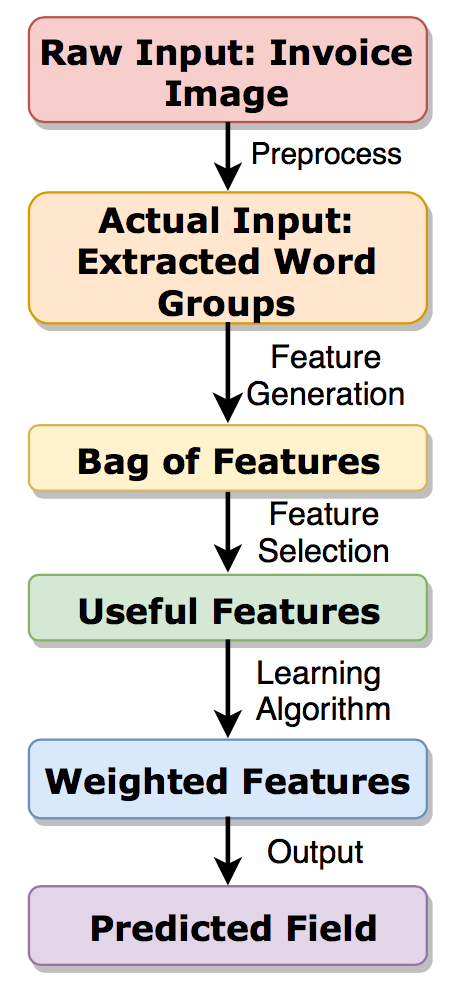
\includegraphics[width=.5\linewidth]{flow_1}
  \caption{Flow of Invoice Recognition}
  \label{fig:flow1}
\end{minipage}%
\begin{minipage}{.5\linewidth}
  \centering
  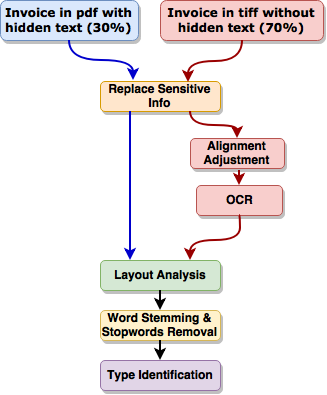
\includegraphics[width=.9\linewidth]{flow}
  \caption{Flow of Data Preprocessing}
  \label{fig:flow2}
\end{minipage}
\end{figure}
